\documentclass[sigconf]{acmart}

% ---- strip ACM copyright/rights boilerplate for a course report ----
\settopmatter{printacmref=false}
\renewcommand\footnotetextcopyrightpermission[1]{}
\setcopyright{none}
\acmConference[MI 2026]{Multimodal Interaction Course Project}{2026}{Rome, Italy}
\pagestyle{plain}

\usepackage{tikz}
\usetikzlibrary{positioning, arrows.meta}
\providecommand{\newblock}{\hskip .11em plus .33em minus .07em}

\begin{document}

\title{SketchTalk: A Multimodal Air-Gesture and Speech Interface for Architecture Diagram Sketching}

\author{Author 1 Name}
\affiliation{%
  \institution{Sapienza University of Rome}
  \country{Italy}}
\email{author1@studenti.uniroma1.it}

\author{Author 2 Name}
\affiliation{%
  \institution{Sapienza University of Rome}
  \country{Italy}}
\email{author2@studenti.uniroma1.it}

\begin{abstract}
Sketching a software architecture diagram usually means a mouse, a
touchscreen, or a pen -- all awkward to reach for while presenting a system
live over a video call, where sketching it on the fly, in view of the same
webcam already running the call, is more natural than switching to a
separate drawing tool, or when a user simply prefers not to touch a
device. SketchTalk lets a user draw boxes and connectors in
the air with a pinch gesture, tracked through a webcam, while an offline
speech recognizer supplies labels, icon choices, and commands such as
connect, delete, undo and export. Neither channel is a complete interface
on its own: gesture always supplies the geometry of what is drawn, while
the meaning of a shape (its label, its type, whether two shapes should be
connected) can come from speech, from a dedicated gesture, or from pointing
combined with a spoken demonstrative, depending on which is more reliable
for that particular action. This report describes the system's
architecture, the specific algorithms used for shape recognition, deictic
reference resolution and connector routing, and the testing done so far.
\end{abstract}

\begin{CCSXML}
<ccs2012>
<concept>
<concept_id>10003120.10003121.10011748</concept_id>
<concept_desc>Human-centered computing~Interaction techniques</concept_desc>
<concept_significance>500</concept_significance>
</concept>
<concept>
<concept_id>10003120.10003121.10003122</concept_id>
<concept_desc>Human-centered computing~Interactive systems and tools</concept_desc>
<concept_significance>300</concept_significance>
</concept>
</ccs2012>
\end{CCSXML}

\ccsdesc[500]{Human-centered computing~Interaction techniques}
\ccsdesc[300]{Human-centered computing~Interactive systems and tools}

\keywords{multimodal interaction, gesture recognition, speech recognition, sketch recognition, deictic reference, hand tracking}

\maketitle

\section{Introduction}

\subsection{Problem context}
Diagramming tools (draw.io, Visio, Lucidchart) are built around a pointer
and a keyboard. That works well at a desk, but it does not match a common
scenario: presenting a system design live during a video call, where the
presenter wants to sketch boxes and connectors on the fly, in view of the
same webcam already used for the call, without switching to a separate
application or reaching for a mouse mid-conversation. Touchless interaction
also matters for accessibility and for settings where touching a shared
device is undesirable. Building a system that lets a person sketch boxes,
connectors and labels purely through hand movement and speech, without a
mouse or keyboard, requires solving two problems that are each hard on
their own: recognizing a hand-drawn shape from noisy webcam-tracked
fingertip coordinates, and recognizing spoken commands from a microphone
with an offline (not cloud-based) speech model, which is markedly less
accurate than commercial cloud ASR.

\subsection{Background}
Multimodal interaction combines two or more input channels -- here, hand
gesture and speech -- so that each can compensate for what the other does
poorly. This principle goes back to Bolt's ``Put-That-There'' system, which
first combined speech with a pointing gesture to resolve references such as
``put that there'' \cite{bolt1980}, and was later formalized by Oviatt, who
argued that a well-designed multimodal interface is not simply two input
methods running in parallel, but a system where each modality is used where
it is actually better suited, and where one can compensate for errors in
the other \cite{oviatt1999}. QuickSet applied this directly to diagram-like
map annotation, fusing speech and pen gestures for military simulation
setup tasks \cite{cohen1997}. SketchTalk follows the same principle:
gesture is always responsible for geometry (a shape's position and size, a
connector's path), while meaning -- a label, an icon, a connect or delete
action -- is assigned to whichever channel is more reliable for that
specific case, including gesture-only fallbacks for exactly the situations
where the offline speech model is weakest.

\subsection{Contributions}
\begin{itemize}
  \item A real-time pinch-to-draw pipeline that recognizes rectangles and
    lines from fingertip trajectories using a \$1 unistroke recognizer
    \cite{wobbrock2007}, with a closure-ratio pre-check (endpoint-averaged
    over several samples, not a single noisy frame) to separate closed
    shapes from open strokes before template matching.
  \item A deictic fusion mechanism that resolves ``this''/``that'' by
    looking up the fingertip position at the exact timestamp Vosk assigns
    to that word, not the end of the sentence, with a bounding-box
    containment check first and a centroid-distance/ambiguity fallback,
    plus a clarification prompt when two shapes are genuinely ambiguous.
  \item A connector-routing algorithm that simplifies the user's drawn
    stroke (Ramer--Douglas--Peucker + axis snapping) and clips it to the
    point where it actually crosses each shape's real boundary --
    generalized to work on a shape's true polygon (e.g.\ a UML decision
    diamond), not just its bounding box, so a connector touches the shape
    it was actually drawn against instead of a rectangle around it.
  \item A deliberately mixed-modality design: two actions that would
    normally require speech (choosing a server icon, connecting two
    shapes) also have a gesture-only path, and one action that was
    originally voice-driven (naming an action/decision UML node, which
    needs an open-ended phrase) was moved to keyboard entry after testing
    showed the offline ASR model was not reliable enough for free-form
    sentences -- a considered trade-off rather than a missing feature.
\end{itemize}

\section{Related Work}
Sketch recognition for diagrams is an established area on its own. Tahuti
recognizes UML class diagrams from pen strokes on a tablet by their
geometrical properties, letting users draw as they would on paper rather
than in a constrained, pre-defined way \cite{tahuti2002}. More recently,
Flowmind2Digital converts photographs of hand-drawn flowcharts and mind
maps into a digital format using keypoint detection, evaluated on a
purpose-built dataset of hand-drawn diagrams \cite{flowmind2024}. Both
systems recognize a diagram after it has been drawn, on paper or a tablet
with a pen; neither operates in real time on free-air hand tracking, and
neither incorporates speech. SketchTalk targets the same class of shapes
(boxes, connectors, and in our case UML activity-diagram nodes) but
recognizes them live, stroke by stroke, from webcam-tracked fingertip
movement, and adds voice as a second channel for everything that is not
geometry.

For the recognition step itself, we use the \$1 unistroke recognizer,
chosen for template matching without any training data, at the cost of
covering a smaller shape vocabulary than a trained classifier would
\cite{wobbrock2007}. For hand tracking, we use MediaPipe Hands, which
extracts 21 3D hand landmarks per frame from a single RGB image without
depth sensing \cite{mediapipe2020}, the same building block used by a
number of existing ``air canvas'' drawing prototypes; those prototypes stop
at raw mid-air line drawing and do not attempt to recognize finished
shapes, connect them, or combine gesture with speech.

For speech, we use Vosk, an offline toolkit built on Kaldi-style acoustic
and language models \cite{kaldi2011}, chosen specifically because it does
not depend on a network connection or a cloud API -- relevant both for
privacy and for reliability during an in-person demo. Recent work on the
same toolkit shows that its accuracy is sensitive to vocabulary and noise
conditions and can be improved with a custom language model
\cite{vosk2025}; we did not train a custom model, and this is consistent
with what we observed empirically: the small generic English model is
dependable for short, closed-vocabulary utterances (a label, a command)
and considerably less so for open-ended, free-form sentences, which
directly motivated moving action/decision node naming to the keyboard
rather than trying to make free-form recognition more robust.

\section{System Architecture}

The system runs as a single desktop application (no client/server split)
built around two parallel input pipelines that both feed a shared diagram
state, as shown in Figure~\ref{fig:architecture}. The gesture pipeline
reads webcam frames, extracts hand landmarks with MediaPipe, tracks the
pinch gesture between thumb and index finger, and buffers the fingertip
trail into a stroke; on release, the stroke is classified as a rectangle
or a line and turned into a \texttt{Shape} in the \texttt{DiagramStore}.
The speech pipeline runs Vosk continuously in a background thread and
yields finalized transcripts with word-level timestamps; each transcript
is parsed into an \texttt{Intent} (label, delete, undo, export) and,
together with fingertip position samples buffered over the last few
seconds, resolved into a concrete action by the \texttt{FusionEngine}.
Both pipelines write into the same \texttt{DiagramStore}, which also owns
connector routing, undo history, and export to SVG.

\begin{figure}[t]
\centering
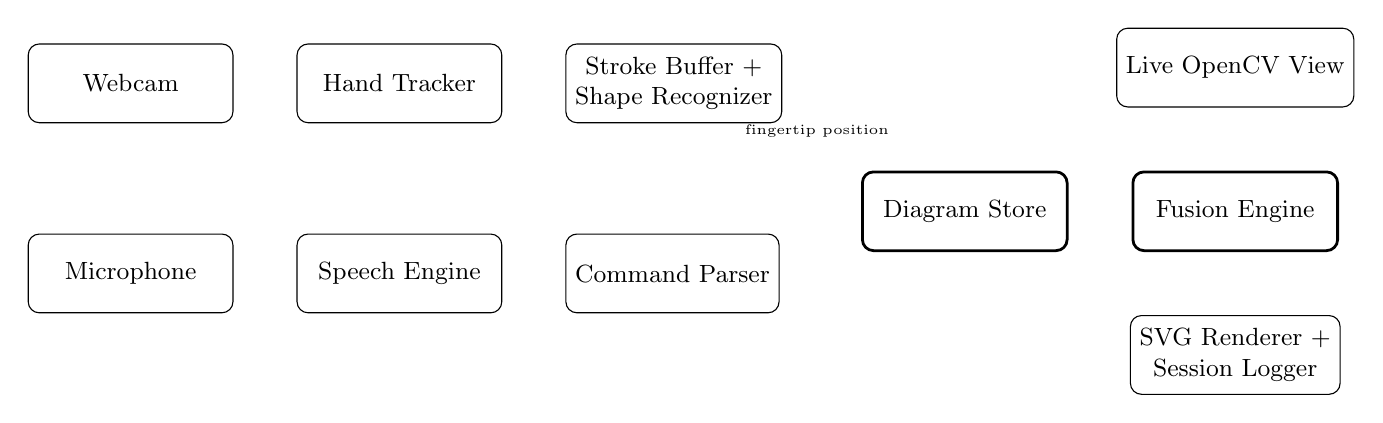
\begin{tikzpicture}[
  node distance=8mm and 8mm,
  box/.style={draw, rounded corners, align=center, minimum width=2.6cm, minimum height=1cm, font=\small},
  emphbox/.style={box, line width=1pt},
  every edge/.style={-{Latex[length=2mm]}}
]
\node[box] (cam) {Webcam};
\node[box, right=of cam] (hand) {Hand Tracker};
\node[box, right=of hand] (shape) {Stroke Buffer +\\Shape Recognizer};

\node[box, below=14mm of cam] (mic) {Microphone};
\node[box, right=of mic] (speech) {Speech Engine};
\node[box, right=of speech] (parser) {Command Parser};

\node[emphbox, below right=6mm and 10mm of shape] (store) {Diagram Store};
\node[emphbox, right=of store] (fusion) {Fusion Engine};

\node[box, above=of fusion] (view) {Live OpenCV View};
\node[box, below=of fusion] (export) {SVG Renderer +\\Session Logger};

\draw (cam) edge (hand);
\draw (hand) edge (shape);
\draw (shape) edge (store);

\draw (mic) edge (speech);
\draw (speech) edge (parser);
\draw (parser) edge (fusion);

\draw (hand) edge[dashed] node[above, font=\tiny]{fingertip position} (fusion);
\draw (store) edge[bend left=15] (fusion);
\draw (fusion) edge[bend left=15] (store);

\draw (store) edge (view);
\draw (store) edge (export);
\end{tikzpicture}
\caption{System architecture. The gesture pipeline (webcam to shape
recognizer) and the speech pipeline (microphone to command parser) both
feed the fusion engine and the shared diagram store, which drives both the
live on-screen view and the SVG exporter.}
\label{fig:architecture}
\end{figure}

% ---- Replace this placeholder with a real screenshot of the running app:
% \begin{figure}[t]
% \centering
% \includegraphics[width=\linewidth]{screenshot.png}
% \caption{Live view: a hand-drawn rectangle labeled ``database'' via voice, with the fingertip overlay visible.}
% \label{fig:screenshot}
% \end{figure}

\section{Implementation}

\subsection{Shape recognition}
Pinch state is derived from the normalized 2D distance between the thumb
and index fingertip landmarks, smoothed over a short moving-average window
to reduce landmark jitter, with separate (asymmetric) thresholds for
starting and releasing a pinch -- drawing a rectangle or circle requires
enough wrist rotation that the apparent thumb-index gap briefly widens
mid-stroke even while the pinch is held, so the release threshold has to
be more forgiving than the start threshold or corners get misread as an
early release.

Once a stroke is finished, its points are resampled and normalized
following the \$1 unistroke algorithm \cite{wobbrock2007} and scored
against two templates (rectangle, line) by finding the best-fit rotation
via golden-section search. Because a rectangle drawn in the air rarely
closes as neatly as one drawn on paper, we gate the classification with a
closure check first: if the (sample-averaged, not single-frame) start and
end points are close relative to the stroke's bounding-box diagonal, the
stroke is treated as closed and scored against the rectangle template;
otherwise it is scored as an open line. This ordering -- closure check
before template matching -- noticeably improved corner-drawn rectangles
being misread as lines, which was the single largest source of
recognition errors observed during development.

\subsection{Deictic fusion}
Resolving ``this''/``that'' to a shape means answering ``where was the
user pointing when they said that word'' rather than ``where are they
pointing now'' -- by the time a phrase is finalized by Vosk, the fingertip
may already have moved on to a different shape. We therefore keep a
rolling buffer of recent $(t, x, y)$ fingertip samples and, for each
deictic word, linearly interpolate the fingertip position at that word's
own start timestamp. That position is first checked against every shape's
bounding box (with a small margin) -- if exactly one shape contains it,
that is treated as an unambiguous match, since pointing at a corner or
edge of a large shape is common and centroid distance alone tends to miss
those cases. If no shape contains the point, the nearest shape by
centroid distance is used instead, provided it is close enough and
clearly closer than the second-nearest candidate; otherwise, the two
closest shapes are offered back to the user as a numbered clarification
prompt.

\subsection{Connector routing}
A connect gesture (a line drawn from inside one shape to inside another)
is turned into a clean orthogonal connector rather than left as the raw,
wobbly stroke. The raw stroke is first simplified with the
Ramer--Douglas--Peucker algorithm and snapped to horizontal/vertical
segments, then trimmed: everything the stroke drew before it left the
source shape's real boundary, or after it first reached the target
shape's boundary, is discarded, since a hand release often drifts a
little further before the pinch is registered as released. The boundary
itself is computed against each shape's actual polygon rather than its
bounding box -- for a plain rectangle these are the same thing, but a UML
decision node is drawn as a diamond inscribed in its bounding box, and
clipping against the bounding box instead of the diamond's real edges
would land the connector's endpoint in the empty triangular gaps between
the diamond and its corners, visibly detached from the shape it was
supposed to touch.

\subsection{Voice, gesture, and keyboard: choosing per action}
Every action in the system was deliberately assigned to whichever input
channel is most reliable for it, rather than defaulting to voice
everywhere or gesture everywhere:
\begin{itemize}
  \item Drawing and connector shape always come from the pinch gesture --
    this is inherently a geometric action that speech cannot express
    directly.
  \item Short labels and fixed keywords (``database'', ``server'',
    ``cloud'', ``action'', ``decision'') are recognized by voice,
    including a small amount of fuzzy matching for near-miss ASR output,
    and by keyword recognition alone the same rectangle can also become a
    server icon via a dedicated gesture (drawing a line inside it), so the
    choice does not depend on speech succeeding.
  \item Connecting two shapes is primarily a gesture (drawing a line
    between them); pointing and saying ``this''/``that'' is available
    too, but is a harder coordination task and is explicitly documented as
    the secondary path.
  \item Naming an action/decision node needs an open-ended phrase, which
    is exactly where the offline ASR model is least reliable -- after
    testing this with real spoken names and seeing frequent
    misrecognition, this step was moved to a small on-screen keyboard
    prompt that opens automatically once a node is awaiting a name,
    confirmed with Enter or cancelled with Escape.
\end{itemize}

\section{Evaluation}
Because the system's correctness depends on the interaction between two
live sensor streams (webcam and microphone), most validation so far has
been iterative, hands-on testing by the two developers across many real
sessions rather than a scripted benchmark. This testing surfaced and led
to fixing several concrete issues: fingertip pinch detection becoming
unreliable near the frame's edges and at shape corners; the connector's
arrow entering a target shape and pointing in the wrong direction because
the routing logic picked up a later, accidental crossing instead of the
first real one; the undo command removing shapes and connectors out of
chronological order; label parsing failing on narrated sentences where the
label word was not at the start of the utterance; and, most recently,
connectors visibly missing a UML decision node's actual diamond boundary.
Each of these was diagnosed from either a screen recording of a failing
case or a printed transcript of what Vosk actually returned, and fixed at
the responsible layer (hand tracking thresholds, connector routing, or
command parsing) rather than patched around.

A short structured pilot with two testers -- covering a fixed list of
scenarios (draw and label each supported shape type, connect two shapes by
gesture and by voice, delete by pointing and by label, undo, export) and
counting first-attempt successes against retries -- is planned as the
final validation step before submission, using the existing per-session
JSON event log (\texttt{session\_logger.py}) to recover objective counts
rather than relying on subjective impressions of the final diagram. This
report reflects the system's state prior to that pilot; \emph{[add results
here once the pilot has been run]}.

\section{Limitations and Future Work}
Fingertip tracking degrades with poor lighting, fast motion, and positions
near the edge of the frame. Offline ASR accuracy drops for longer or less
common phrases, which is why several interactions were deliberately moved
off voice (gesture-only server icon and connect, keyboard entry for node
names) rather than trying to force voice to cover everything. The system
currently recognizes two shape types (rectangle, line) plus two UML node
types (action, decision); a richer shape grammar, and the currently unused
\texttt{GESTURE\_ONLY}/\texttt{SPEECH\_ONLY} ablation modes referenced in
the configuration, are left for future work. There is also no
single-utterance voice command for connecting two shapes (``connect this
to that'') -- the coordination it requires (moving the pointing finger in
sync with two words in one sentence) proved too fragile in testing and was
removed in favor of the gesture-only connect and a two-step pointing
fallback.

\section{Conclusion}
SketchTalk combines real-time pinch-gesture shape recognition with offline
speech recognition into a single hands-free diagramming tool, with an
explicit design principle -- gesture for geometry, whichever channel is
more reliable for meaning -- rather than treating either modality as a
strict primary. The main technical contributions are the closure-gated
shape recognizer, the timestamp-synchronized deictic fusion mechanism, and
a connector-routing algorithm that clips against a shape's real drawn
boundary rather than its bounding box. Development-time testing already
surfaced and fixed a number of concrete failure modes; a short structured
two-person pilot remains to close out the evaluation before submission.

\begin{thebibliography}{9}

\bibitem{bolt1980}
Richard A. Bolt. 1980.
\newblock ``Put-That-There'': Voice and Gesture at the Graphics Interface.
\newblock \emph{ACM SIGGRAPH Computer Graphics} 14, 3, 262--270.

\bibitem{oviatt1999}
Sharon Oviatt. 1999.
\newblock Ten Myths of Multimodal Interaction.
\newblock \emph{Communications of the ACM} 42, 11, 74--81.

\bibitem{cohen1997}
Philip R. Cohen, Michael Johnston, David McGee, Sharon Oviatt, Jay Pittman,
Ira Smith, Liang Chen, and Josh Clow. 1997.
\newblock QuickSet: Multimodal Interaction for Distributed Applications.
\newblock In \emph{Proceedings of the Fifth ACM International Conference on
Multimedia}, 31--40.

\bibitem{wobbrock2007}
Jacob O. Wobbrock, Andrew D. Wilson, and Yang Li. 2007.
\newblock Gestures without Libraries, Toolkits or Training: A \$1
Recognizer for User Interface Prototypes.
\newblock In \emph{Proceedings of UIST 2007}, 159--168.

\bibitem{tahuti2002}
Tracy Hammond and Randall Davis. 2002.
\newblock Tahuti: A Geometrical Sketch Recognition System for UML Class
Diagrams.
\newblock In \emph{AAAI Spring Symposium on Sketch Understanding}, 59--66.

\bibitem{flowmind2024}
Huanyu Liu, Jianfeng Cai, Tingjia Zhang, Hongsheng Li, Siyuan Wang,
Guangming Zhu, Syed Afaq Ali Shah, Mohammed Bennamoun, and Liang Zhang.
2024.
\newblock Flowmind2Digital: The First Comprehensive Flowmind Recognition
and Conversion Approach.
\newblock arXiv:2401.03742.

\bibitem{mediapipe2020}
Fan Zhang, Valentin Bazarevsky, Andrey Vakunov, Andrei Tkachenka, George
Sung, Chuo-Ling Chang, and Matthias Grundmann. 2020.
\newblock MediaPipe Hands: On-device Real-time Hand Tracking.
\newblock arXiv:2006.10214.

\bibitem{kaldi2011}
Daniel Povey, Arnab Ghoshal, Gilles Boulianne, et al. 2011.
\newblock The Kaldi Speech Recognition Toolkit.
\newblock In \emph{IEEE Workshop on Automatic Speech Recognition and
Understanding (ASRU)}.

\bibitem{vosk2025}
Aniket Abhishek Soni. 2025.
\newblock Improving Speech Recognition Accuracy Using Custom Language
Models with the Vosk Toolkit.
\newblock arXiv:2503.21025.

\end{thebibliography}

\end{document}
